\documentclass[i2]{oss}
\setlength{\topmargin}{-.5in}
\setlength{\textheight}{9in}
\setlength{\oddsidemargin}{.100in}
\setlength{\textwidth}{6.25in}
\usepackage[english]{babel}
\usepackage{graphicx}
\usepackage{amsmath}
\usepackage{fullpage}
\usepackage{color}
\usepackage{soul}
%\usepackage{gensymb}
\usepackage{caption}
\usepackage{subcaption}
\usepackage[section]{placeins}

\newcommand{\class}[1]{\emph{#1}}
\newcommand{\method}[1]{\emph{#1}}
\newcommand{\junit}{\emph{JUnit }}
\newcommand{\comment}[1]{{\huge \textcolor{green}{#1}}}

\begin{document}

\members{Joren Verspeurt {\small \texttt{(r0258417)} } \\
         Sophie Marien {\small \texttt{(s0216517)}}\\
         Stef Noten {\small \texttt{(s0211264)}}\\
         Toon Nolten {\small \texttt{(r0258654)}} \\
         Begeleider: Mario H. C. T.} % teamleden

\maketitlepage
\newpage
\tableofcontents
\pagebreak




%-----------------------------------------------------------------------
%	INLEIDING
%-----------------------------------------------------------------------
\section*{Introduction}
\label{ssec:introduction}
%introductie en de belangrijkste elementen van ons ontwerp
%test
Unit Tests are important because today's software systems are very 
complex.
\emph{junit} is the most popular framework for unit testing in the Java 
language.
Currently running the tests is either done manually by developers or
automatically by a continuous integration tool on a central server.
A disadvantage of these approaches is that tests only run when a 
developer decides to or when a developer commits work to the central 
repository.
This can be improved by using a daemon (background process) that continuously runs tests, this gives the developer rapid feedback and 
takes away the burden of manually starting tests.


%TODO Design strategy/... summary?


%-----------------------------------------------------------------------
%	ONTWERP
%-----------------------------------------------------------------------
\section{Design}
\label{ssec:design}
%Klassendiagram en interactie diagrammen

In this section we describe how our design followed from an analysis
of responsibilities and we go through the start-up and execution of 
our application.

\subsection{Design and responsibilities}

The guiding principle for our design is a clear separation of 
responsibilities. The first step is an analysis of necessary actions:

\begin{itemize}
	\item Run tests
    \item Collect information on tests
    \item Summarize the available information for a test
    \item Order tests according to a user-specified policy
    \item Output of results
\end{itemize}

Each of these is different enough to merit an entire entity responsible 
for that action. Those entities were implemented as \emph{Daemon},
\emph{DataCollector}, \class{Statistic}, \class{Policy} and
\class{ConsoleView}. Our daemon makes as much use of the existing \junit
infrastructure as possible. We only needed to extend three existing
classes: \class{FlattenedRequest} is a request that contains only tests
(no suites) as children (this was basically copied from \class{MaxCore} 
in the experimental package), \class{MethodRunner} was necessary because
when sorting a \class{FlattenedRequest} the description of the children
was actually the description of the testclass containing the method and
not the method itself, \class{RunNotificationSubscriber} does not extend
anything from \junit but is used as a protection proxy so \class{Daemon}
does not have to pass an actual \class{RunNotifier} which could be used
to fire events (testRunStarted, testFailed...).

The \class{Daemon} is responsible for running tests.
It can make use of different \class{Policy}'s to order the tests that 
need to be run.

A \class{Policy} could do many different things, we use them only for
ordering tests but they could also filter requests or (? nog iets).
% (this filtering is not implemented in the current state of the application but is a possible extension).
A \class{SortingPolicy} makes use of \class{Statistic}'s to determine
an order for tests
At the moment the following policies are supported: last failure first, 
frequent failure first, distinct failure first and changed code 
first.
Each of these determines a different order that can be useful for
developers.
For example, tests that consistently order first under the frequent
failure first policy might indicate brittle/(badly written) code.

\class{Statistic}'s calculate any necessary information for the ordering
of tests from data collected by dedicated \class{DataCollector}'s.
Examples of data that has to be collected: every failure of a test,
which code a test depends on and what code changes.

% Deze subsecties mogen er wel bij vindt ik, miss nog een paar meer.
\subsubsection{Collecting statistics}
To enable handling tests in different ways according to different events 
that can occur during testing (like failures, changes to class files) 
a number of different statistics need to be gathered.
Supported

\subsubsection{Collecting data for statistics}





\begin{description}
\item Collecting Statistics.( rejecting of the statistic pool)
At the beginning of the brainstorm of the design we included a class {Statistic Pool}. This class would have kept all the statistics. By a request there will be checked if it owns a specific statistic. If the requested statistic is not owned by the \emph{StatisticPool} then the statistic will be registered. This was eventually rejected because there would be too much dependently on this class. Statistics are still being kept but this is now done in the \emph{StatisticManager}.
%TODO is dit correct?

\item Policies
Composite filters and sorting policies.
A \emph{Policy} has an apply. This apply will operates on a request and it will return a request. In addition, every policy has a child as Policy. If an apply is called, then it will first call the apply of the child and after that it will call its own apply on the resulting request. We can not guarantee that the result is correct according to the multiple sorting policies that are done. SortingRequest can not be applied over multiple levels (if there is a filterRequest in between). The assumption we are making here is that the new sorting will wipe out the older sorting instead of putting it together.
%TODO dit was veranderd naar een ander ontwerp

\item Collectors
For \emph{FailureTraceCollector} are the parallel tests not supported. This is not supported because it will take a lot of time to implement it and there are other priorities.
\end{description}

%-------------KLASSENDIAGRAMMA------------------------------------------
\subsection{Klassendiagramma}
\label{ssec:Klassendiagramma}

Each class has its own well-defined set of responsibilities.

\begin{description}

\item \emph{Daemon}: \emph{Daemon} is responsible for initializing the 
application. It provides an interface to set a policy for presenting 
test results according to statistics gathered during test runs.

\item \emph{DataCollector}: A \emph{DataCollector} is responsible for
collecting specific kinds of data. These data can be related to test
execution or changes that occur to the test environment such as changed
files.

\item \emph{DataEnroller}: The \emph{DataEnroller} provides the service
of subscribing //TODO

\item \emph{Policy}:\emph{SortingPolicy} is responsible for the ordering of tests by a certain policy and it can also implement a filter for a \emph{FilterPolicy} so it can also filter certain tests.

\item \emph{Statistic}: \emph{Statistic} is responsible for the calculations of statistics based on the data that is collected through the \emph{Data}class

\item \emph{StatisticProvider}: 

\item \emph{DataEnroller}: 



\end{description}


%figuur oud klassendiagram
\begin{figure}[tbp]
\begin{center}
    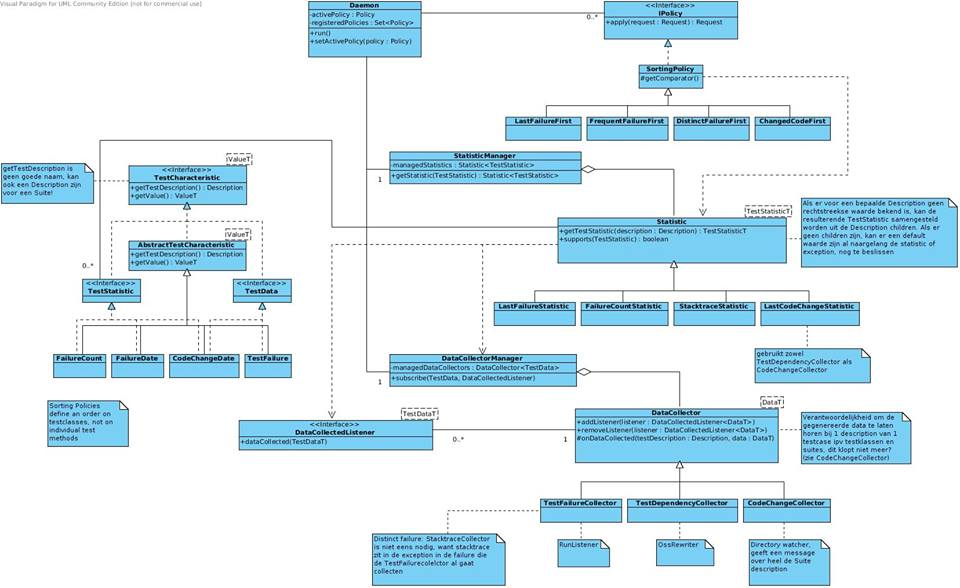
\includegraphics[width=0.8\textwidth]{klassendiagramOud}
    \caption{The old classdiagram}
	\label{fig:kd-oud}
\end{center}
\end{figure}



%figuur nieuw klassendiagram
\begin{figure}[tbp]
\begin{center}
    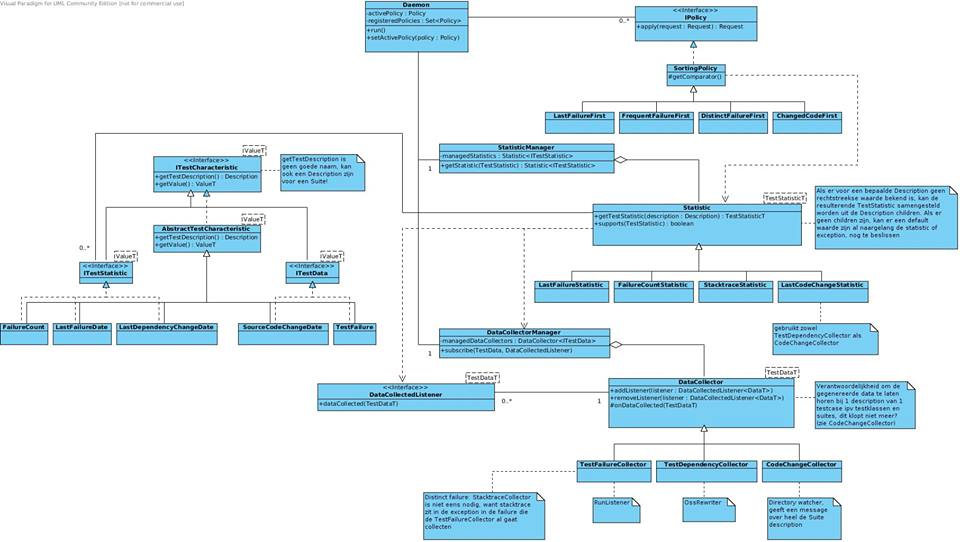
\includegraphics[width=0.8\textwidth]{klassendiagram}
    \caption{The intermediate classdiagram}
	\label{fig:kd-tt}
\end{center}
\end{figure}




%figuur nieuw klassendiagram
\begin{figure}[tbp]
\begin{center}
    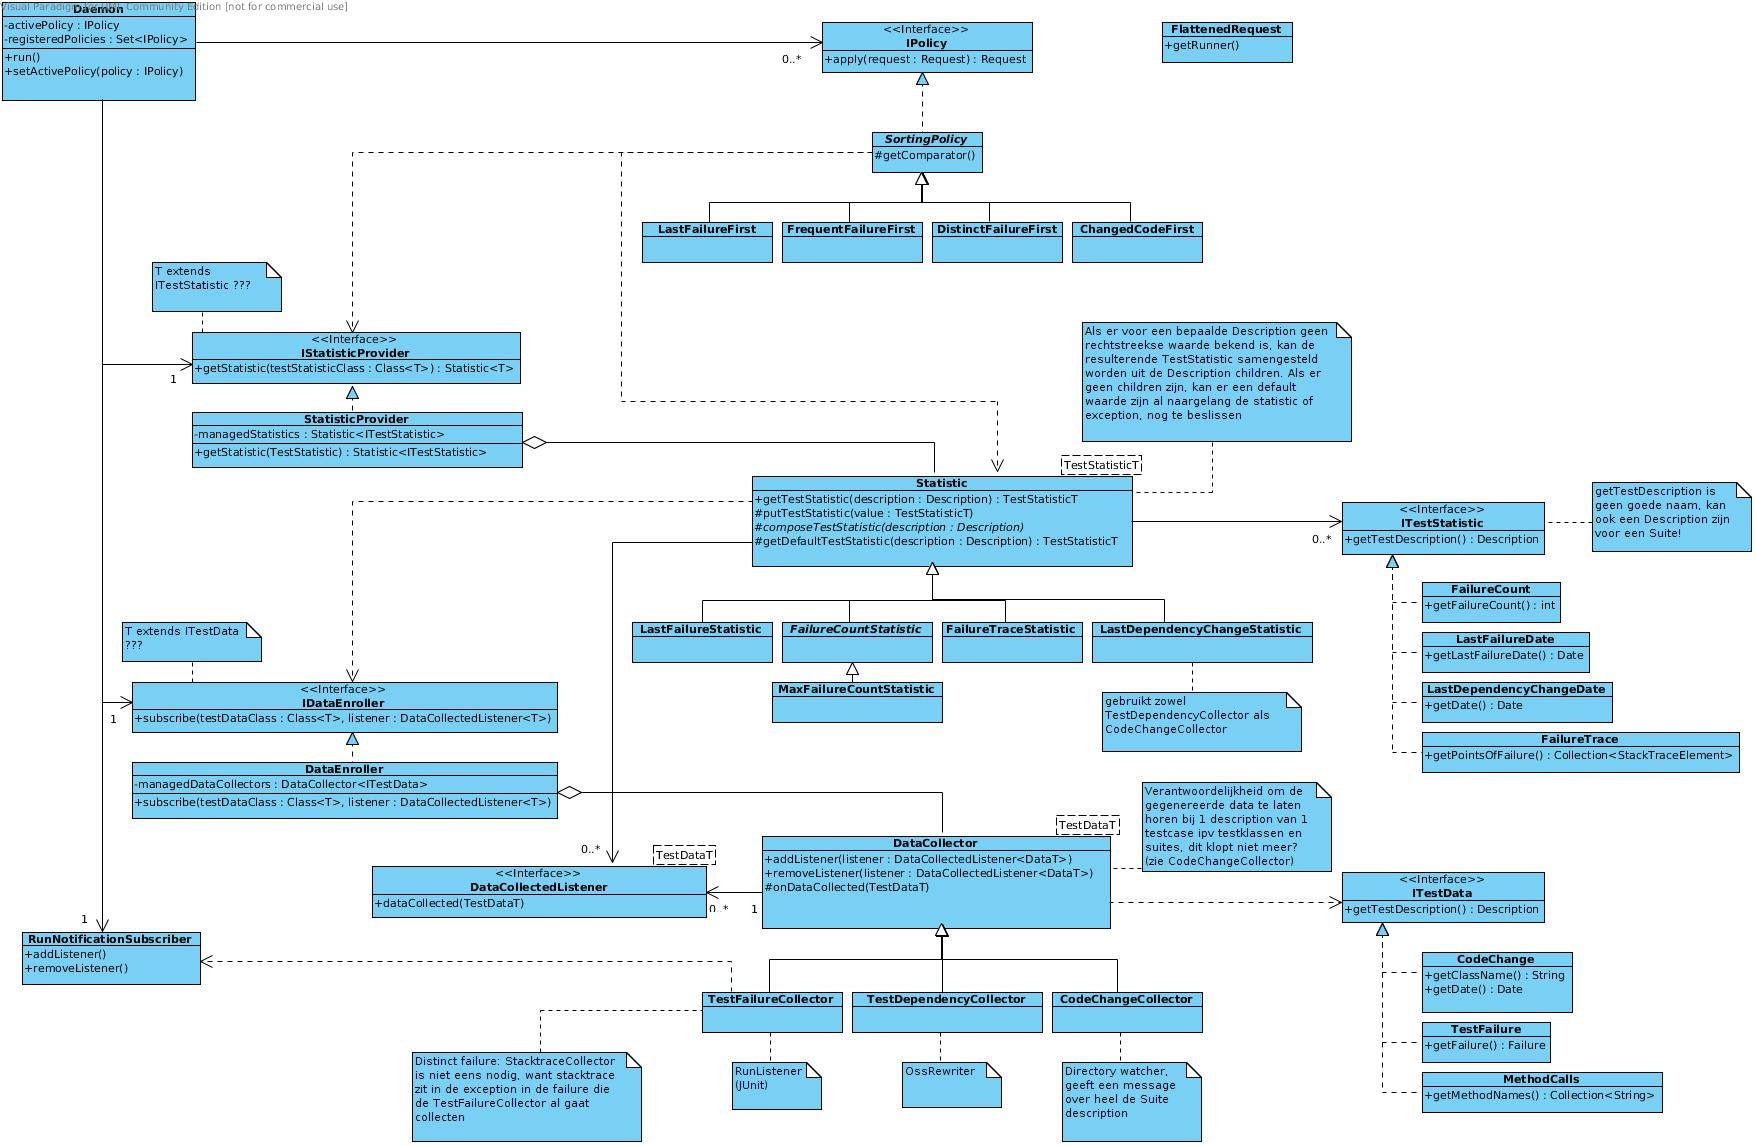
\includegraphics[width=0.8\textwidth]{klassendiagram3}
    \caption{Current classdiagram}
	\label{fig:kd-h}
\end{center}
\end{figure}


%-------------Interactie Diagrammas-------------------------------------
\subsection{Interactie diagrammen}
\label{ssec:Interactiedia}








%

%-----------------------------------------------------------------------
%	TESTEN
%-----------------------------------------------------------------------
\section{Tests}
\label{ssec:tests}
%Een hoofdstuk rond testen dat de procedure beschrijft die gevolgd werd bij het testen: wat
%werd getest en hoe?


%----------------------------------------------------------------------------------------
%	PROJECT MANAGMENT
%----------------------------------------------------------------------------------------
\section{Project management}
\label{ssec:Projectmanag}
%taakverdeling elk lid en welke taak
%uren

%TODO tekst

%TODO laatste week aanvullen!!
\begin{table}[h!]
\begin{center}
    \begin{tabular}{ r | c  c  c  c  c  c}
     & Joren & Toon & Stef & Sophie \\ \hline
    Algemeen & 2u00 & 2u00 & 2u00 & 2u00\\
           Tools & 8u30 & 8u30 & 8u00 & 4u30 \\
        Analyse & 10u00 & 10u00 & 12u15 & 12u00 \\
        Ontwerp & 00u00 & 00u00 & 00u00 & 00u00 \\
        Implementeren & 00u00 & 00u00 & 00u00 & 00u00\\
        Verslag & 9u00 & 9u00 & 9u00 & 9u00 \\
        Totaal & 29u30 & 29u30 & 31u15 & 27u30  
    \end{tabular}
    \caption{Overzicht werkuren per onderdeel}
    \label{tab:werkuren}
\end{center}
\end{table}

%TODO figuren updaten
\begin{figure}[h!]
        \centering
        \begin{subfigure}[hb]{0.20\textwidth}
                \centering
                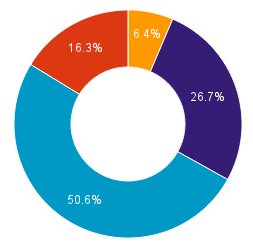
\includegraphics[width=\textwidth]{chart_2}
                \caption{Joren}
        \end{subfigure}%
        \begin{subfigure}[hb]{0.20\textwidth}
                \centering
                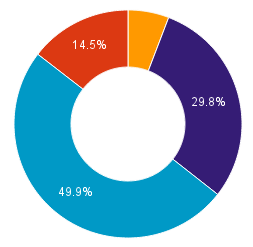
\includegraphics[width=\textwidth]{chart_3}
                \caption{Toon}
        \end{subfigure}%
        \begin{subfigure}[hb]{0.20\textwidth}
                \centering
                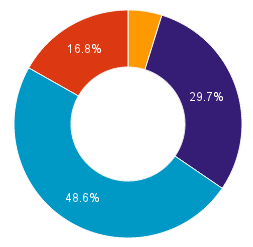
\includegraphics[width=\textwidth]{chart_4}
                \caption{Stef}
        \end{subfigure}%
        \begin{subfigure}[hb]{0.20\textwidth}
                \centering
                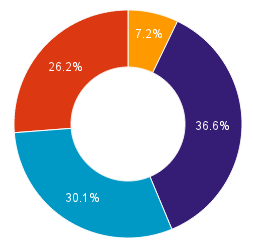
\includegraphics[width=\textwidth]{chart_5}
                \caption{Sophie}
        \end{subfigure}%
                \begin{subfigure}[hb]{0.20\textwidth}
                \centering
                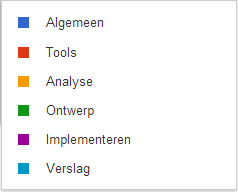
\includegraphics[width=\textwidth]{legende}
                \caption{Legende}
        \end{subfigure}%


 \caption{Weergave van de werkverdeling}
\label{fig:werkverdeling}
\end{figure}





%----------------------------------------------------------------------------------------
%	 CONCLUSIE en DISCUSSIE
%----------------------------------------------------------------------------------------
\section{Conclusie}
\label{ssec:Conclusie}
% Een hoofdstuk met een discussie en conclusie waarin interessante ervaringen, problemen en
%andere opmerkingen omtrent het project worden beschreven



%----------------------------------------------------------------------------------------
%	GLOSSARY
%----------------------------------------------------------------------------------------
\section{Glossary}
\label{ssec:glossary}


Daemon met een policy en een testinformation Klasse en een Statistic information 

Pattern Model-View-Controller
View:  GUI, CLI, passive view
Controller:
Input besturingsview, handeld input/output
Model: Daemon, Policy, TestInfomation, DataCollector, Statistic, TestRun
Daemon is bedoeld als interface voor het model

Verantwoordelijkheden
Policy: ordening, filtering
Statistic: berekent de statistieken, legt een strategie vast om data op te vragen.
TestInformation:  Houdt de statistieken bij (alles dat uit de collectors wordt opgevraagd)
DataCollector: Data verzameling, inpluggen in een TestRun, change code bijhouden (apart in een andere Collector)
Daemon:  Starten van TestRuns
TestRun:  runnen van testen

Implementaties:
Policy als Composit/Decorator/Strategy
We weten niet zeker of het een composit is want er werd getwijfeld tussen Composit en Decorator Pattern. 
Statistic en DataCollector zijn een Strategy
TestInfomation
Eerst mapte Description met een lijst van tuples. Dit is veranderd naar TestSummary
Map<Description,OrderedSet<TestSummary>>
	TestSummary	-Map<Collector, Object>
			- TestID


We streven voor low-coupling. 

Verslag: beginnen met de analyse van wat we nodig hebben en daarna uitleggen hoe we dit oplossen en analyseren en bediscussiëren.

 


\end{document}



